\chapter{Introduction}

%When you think of solids, you generally think of crystals. You take a liquid, and let it cool down, and it falls into a nice crystal structure that is spatially optimized in some way. This is generally how most solids form and is conceptually pretty easy to understand. Glass however can be formed by cooling down a liquid too quickly to find its minimum energy configuration - it essentially just gets stuck in some non-optimal state instead. 

Anyone who has stacked oranges knows that it is easy and intuitive to stack them closely in a dense lattice, as demonstrated in figure \ref{plot:oranges}(a). Filling about $74\%$ of space, the close packed lattice is in fact the densest possible arrangement of equal sized spheres in 3 dimensions. This was originally conjectured by Kepler in 1611 \cite{kepler_strena_1611}, but was not formally proven until 1998 \cite{hales_overview_1998}. If one simply pours them together, they will instead arrange themselves in an amorphous (i.e. random) and less dense structure, as shown in figure \ref{plot:oranges}(b). This amorphous configuration is significantly less efficient, filling only about $64\%$ of space. The lazy but innovative produce worker may attempt to create a close lattice by randomly pouring oranges into a box and squeezing, but experience dictates that this is impossible. The fruit are too much in each other's way to rearrange and relieve the stress from the squeezing. Interestingly, 2 dimensional discs of equal size do spontanously form hexagonal lattices when squeezed, but even discs of nonuniform size generally become frustrated and arrange amorphously.

\begin{figure}[b!]

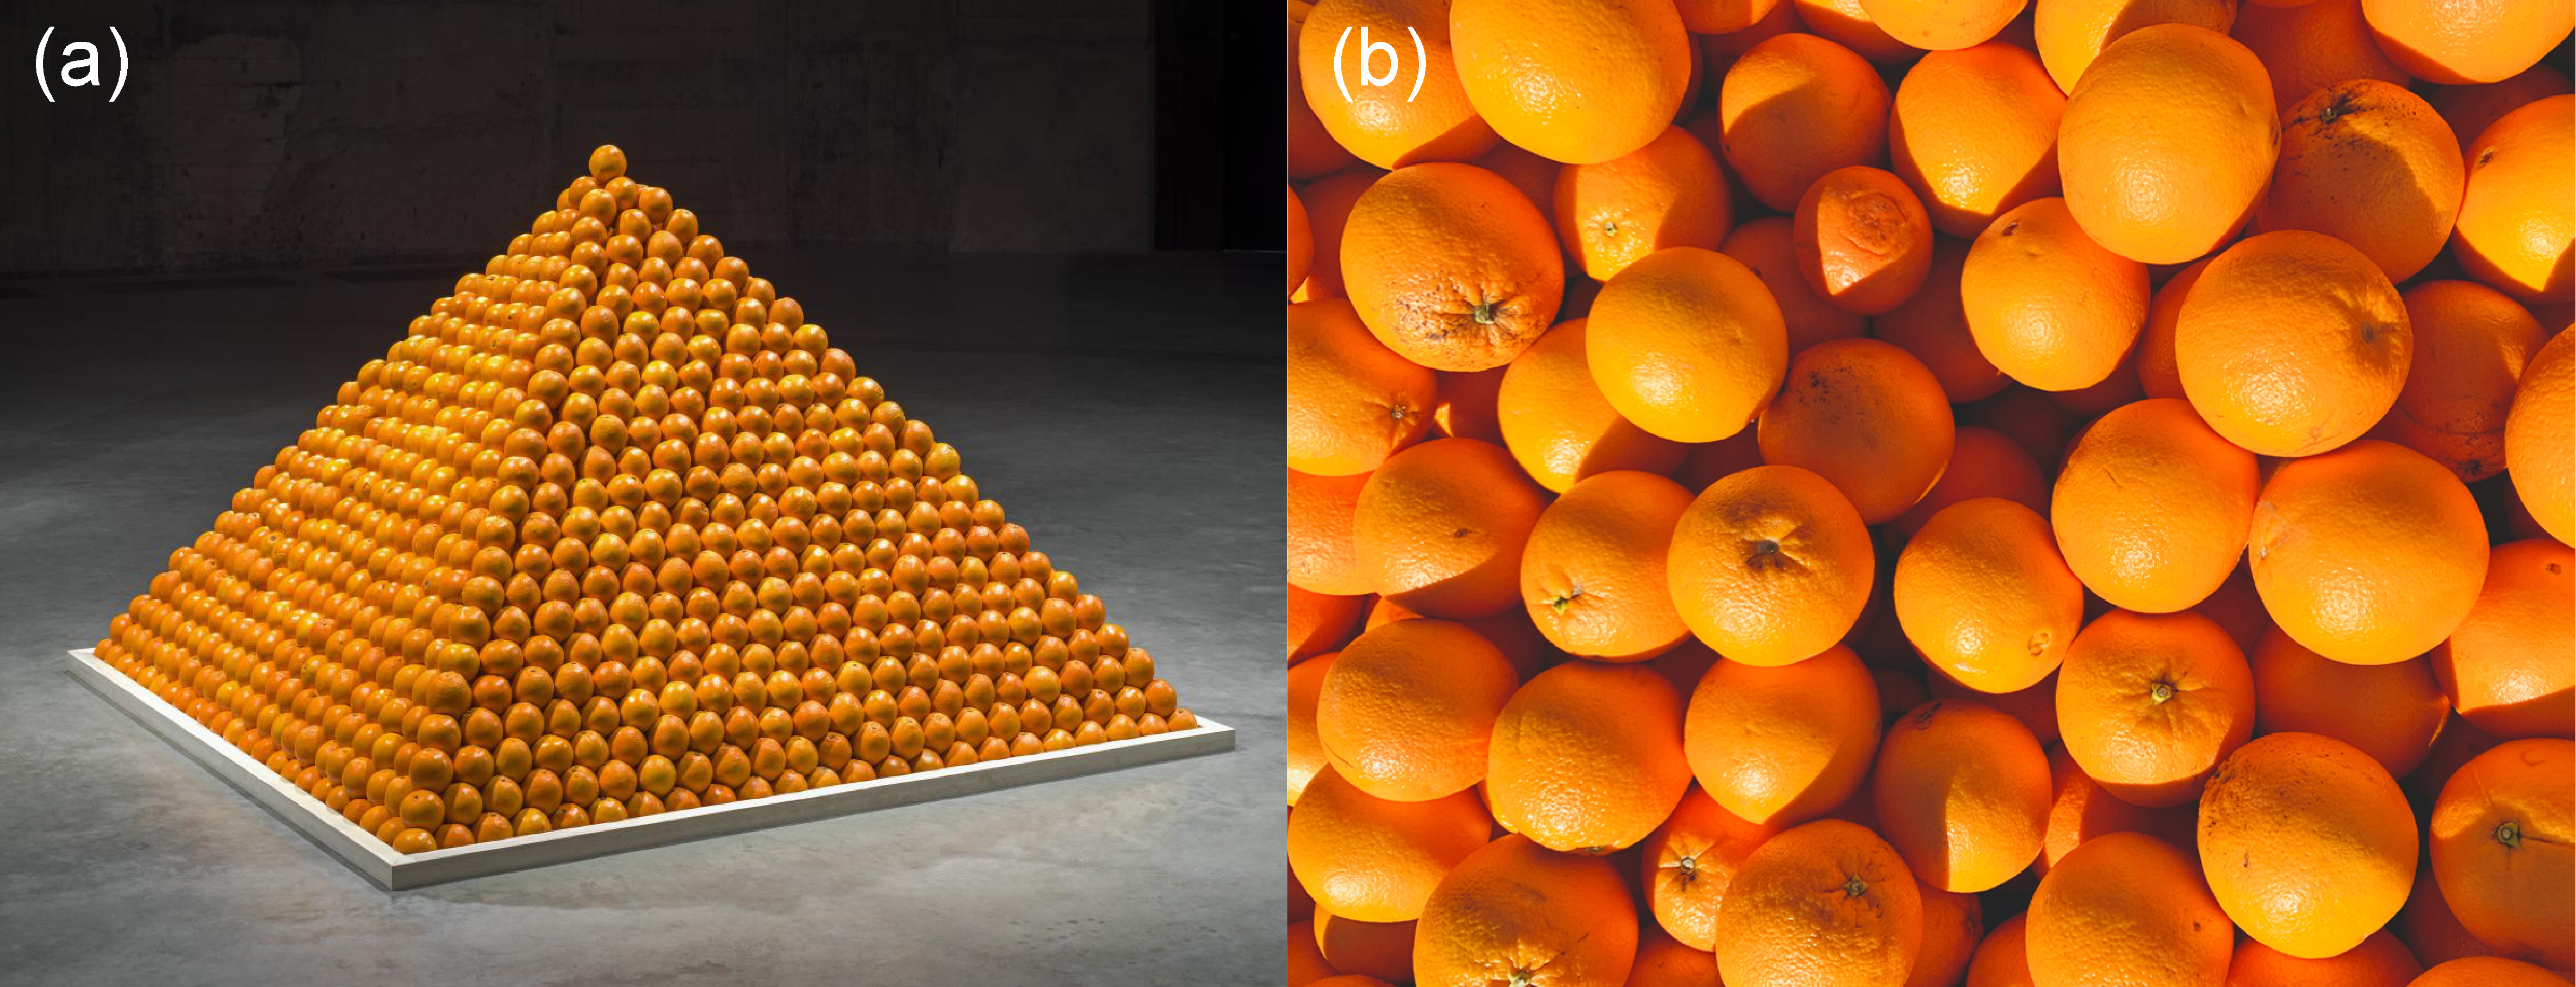
\includegraphics[width=\columnwidth, trim=0 0 0 0, clip]{oranges.pdf}

\caption[Left, stack of oranges constructed in a close packed lattice \cite{louw_soul_1967}. Right, oranges arranged amorphously \cite{gunter_photo_2021}.]{Left, stack of oranges constructed in a close packed lattice \cite{louw_soul_1967}. Right, oranges arranged amorphously \cite{gunter_photo_2021}.}
%https://unsplash.com/photos/A4BBdJQu2co
%https://www.tate.org.uk/art/artworks/louw-soul-city-pyramid-of-oranges-t13881

\label{plot:oranges}
\end{figure}

Granular materials are collections of distinct macroscopic objects, such as sand, ball bearings, or piles of oranges. While crystalline structures such as close lattices are relatively straightforward to understand and analyze, the random features of amorphous granular systems make them extremely difficult to understand from first principles. The only analytic approach that has been somewhat successful requires taking the limit of infinite spatial dimensions, termed ``mean field.'' Since all physical systems are finite dimensional, results from the mean field limit do not necessarily apply. Many results from the mean field are however surprisingly accurate even in as low as 2 and 3 dimensions. Our research is not focused on analytic theory, but rather on computational study of soft spheres, i.e. spheres which are able to interact with their neighbors, imparting variable forces upon them. %Although the forces between granules of physical systems arise from physical deformations, this can be approximated with non-deforming but slightly overlapping spheres. 
In general when one simulates systems in greater than three dimensions, the purpose is to draw parallels with results from the mean field.


A phase transition is when a material undergoes a discontinuous change in some property (the ``order parameter'') as some other property (the ``control parameter'') varies. The most well known phase changes are freezing/melting and boiling/condensing, for which the temperature is the control parameter, and the density of the material can be seen to discontinuously change at critical temperatures. The order parameter is generally accepted to be the free energy - at the phase transition, melting absorbs a latent heat in addition the heat required just to heat it to the melting point. While glasses go through thermal phase transitions, granular materials do not, because thermal fluctuations are insufficient in scale to allow rearrangement of grains. For example, take the box of oranges discussed earlier: thermal fluctuations (providing energy $E \sim kT \sim 0.026$ eV) cannot cause a pair of oranges to rearrange (requiring $E \sim mgh \sim 10^{17}$ eV). Granular materials are thus described as ``athermal'' or ``zero-temperature.''  Granular materials do however go through a different type of transition, called the jamming and unjamming transitions, which are somewhat analogous to thermodynamic phase transitions. The control parameter for the jamming transition is the fraction of space occupied by particles, or packing fraction $\varphi$, and the jamming transition happens at a critical packing fraction $\varphi_J$, where properties of the system go through discontinuous changes. In particular, the pressure $P$ begins to increase from 0, and the number of force bearing contacts between granules goes from 0 to roughly the number of particles times the spatial dimension $Nd$. The critical packing fraction is an exact value for any particular system, but generally has some variation between systems, and can vary based on the protocol of system generation. The jamming point can be understood as a critical point, and as the system increases in packing fraction from that point, properties such as the number of contacts in excess of Nd, the pressure, and the packing fraction in excess of $\varphi_J$ all scale with each other as power laws \cite{ohern_jamming_2003,goodrich_scaling_2016}.

Traditional approaches to analyzing thermodynamic systems rely on the assumption of ergodicity, i.e. that the thermal system explores the ensemble of all available configurations. The probability of existing in any particualar configuration is determined by the ratio of the energy of that configuration with the temperature of the system. In a zero temperature granular material, however, this is obviously impossible. Despite this, granular materials do respond predictably to repeated disturbances, e.g. if you repeatedly shake a box of rocks, they will reliably settle into a configuration of roughly the same packing fraction. Thus, some version of athermal statistical mechanics is clearly at work. In 1989 Sam Edwards began a systematic attempt at understanding granular materials in thermodynamic terms \cite{edwards_theory_1989}. ``Angoricity,'' which relates entropy to pressure rather than energy is derived from this work and has shown promise as a temperature analog for granular materials \cite{edwards_distribution_2008,bi_statistical_2015}. 

The jamming transition identifies the onset of rigidity. Below $\varphi_j$, a system is floppy and unable to sustain any force. Above $\varphi_j$ however a system becomes rigid and can support external forces. You can run your hands through sand at the beach, but if you compress it, it will push back. This rigidity can be understood in terms of degrees of freedom and constraints - it arises when the system has at least as many constraints as degrees of freedom. A system where these are exactly equal is termed ``isostatic,'' and a system with more constraints than degrees of freedom is termed ``hyperstatic.'' Since each particle can move in $d$ dimensions, a granular system has $Nd$ degrees of freedom. The constraints on those degrees of freedom are the contacts between particles, which increase in quantity with increasing packing fraction or pressure. The jammed configurations under inquiry are hyperstatic and thus are rigid and may support external forces. When considering instead the force network of the system, each contact is a degree of freedom, and requiring force balance on each particle imposes $Nd$ constraints. Thus while the positions of particles in a hyperstatic system is overdetermined, the force network supporting this rigidity is underdetermined. There exists a degerate space of allowed force configurations, which is referred to as the Force Network Ensemble or FNE \cite{snoeijer_force_2004,tighe_force_2010}. This Force Network Ensemble framework forms the basis for the majority of the material in this work.

The following three chapters are the three first author papers which I composed during my time as a graduate student. Chapter \ref{forceVolumeEntropyPaper} (published in PRE \cite{sartor_direct_2020}) explores a method that I developed along with Eric Corwin that uses the Force Network Ensemble to measure the allowed space of force configurations for a granular system. This allowed us to measure the entropy of the force networks for the first time from the microscopic structure. We confirm this entropy measurement by comparing it with a bulk measurement of angoricity, concretely linking it with the microscopic multiplicity of the Force Network Ensemble. In Chapter \ref{contactBreaking} (in review \cite{sartor_predicting_2021}), we use a similar approach to examine the boundaries of the allowed space of force configurations. These boundaries correspond to systems with fewer contacts than the original system. By examining which contacts are missing in those boundary systems, we are able to predict which contacts between particles are unnecessary. We then show that only these defect contacts may in fact be broken under decompression. These force network defects are a completely new form of defect in amorphous materials. In chapter \ref{excessContactsScaling} (published in PRL \cite{sartor_mean-field_2021}), working with Eric Corwin and Sean Ridout, we closely examine the relation between critical scaling laws about the jamming transition. Rather than just looking at the well known exponents of these scaling laws, we delve deeper and explore the prefactors to these scaling laws. Although pefactors such as these are generally highly sensitive to finite dimensional corrections, we show that they are still well predicted by the mean field. We provide a first principles proof for one free of the mean field assumption, demonstrating that mean field theory is not necessary for explaining scaling laws in low dimensional jamming.
